\section{Risultati e osservazioni}
\begin{frame}{Risultati}
    \begin{center}
        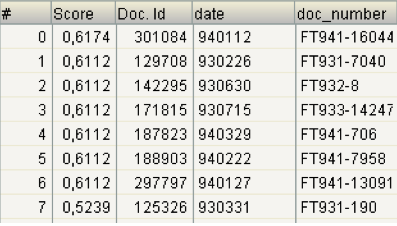
\includegraphics[width=0.5\textwidth]{img/luke-2.png}

        \bigskip
        La più semplice query con Luke.

        `from' è la parola con la frequenza più alta nella collezione.
    \end{center}
\end{frame}
\begin{frame}{Risultati}
    \begin{columns}
        \begin{column}{0.5\textwidth}
            \begin{table}[H]
                \centering
                \fontsize{6}{6}\selectfont
                \begin{tabularx}{\columnwidth}{YYYY}
                    \toprule
                    \textbf{Topic Set}             & \textbf{MAP}            & \textbf{GMAP}             & \textbf{RECALL}         \\
                    \midrule
                    \multirow{2}*{\textit{TREC-6}} & 0.2148                  & 0.0761                    & 0.4778                  \\
                                                   & \textcolor{red}{0.1612} & \textcolor{green}{0.0843} & \textcolor{green}{0.5382} \\
                    \midrule
                    \multirow{2}*{\textit{TREC-7}} & 0.1771                  & 0.0706                    & 0.4867                  \\
                                                   & \textcolor{red}{0.1734}                  & \textcolor{green}{0.0843}                    & \textcolor{green}{0.5444}                  \\
                    \midrule
                    \multirow{2}*{\textit{TREC-8}} & 0.2357                  & 0.1316                    & 0.5895                  \\
                                                   & \textcolor{red}{0.1899}                  & \textcolor{red}{0.0906}                    & \textcolor{red}{0.5484}                  \\
                    \midrule
                    \multirow{2}*{\textit{Robust}} & 0.2555                  & 0.1290                    & 0.7715                  \\
                                                   & \textcolor{red}{0.2021}                  & \textcolor{red}{0.1016}                    & \textcolor{red}{0.6052}                  \\
                    \bottomrule
                \end{tabularx}
            \end{table}
            \fontsize{6}{6}\selectfont Risultati di LM di base
        \end{column}
        \begin{column}{0.5\textwidth}
            \begin{itemize}
                \item Indicizzazione con la stoplist standard di Lucene
                \item Parser standard di Lucene per ottenere query su cui trovare metriche
                \item Uso di uno stemmer? Improbabile...
            \end{itemize}
        \end{column}
    \end{columns}
\end{frame}
\begin{frame}{Considerazioni finali}
    \begin{itemize}
        \item GLM migliore di LM
        \item Per ottenere i knn serve molto tempo
        \item Risultati non riprodotti
        \item Tempo sottostimato per implementare gli step necessari per riprodurre i risultati del paper
        \item È stato usato solo Lucene perché è quanto viene usato secondo il paper.
    \end{itemize}
\end{frame}